\begin{center}
\begin{figure}[h]
	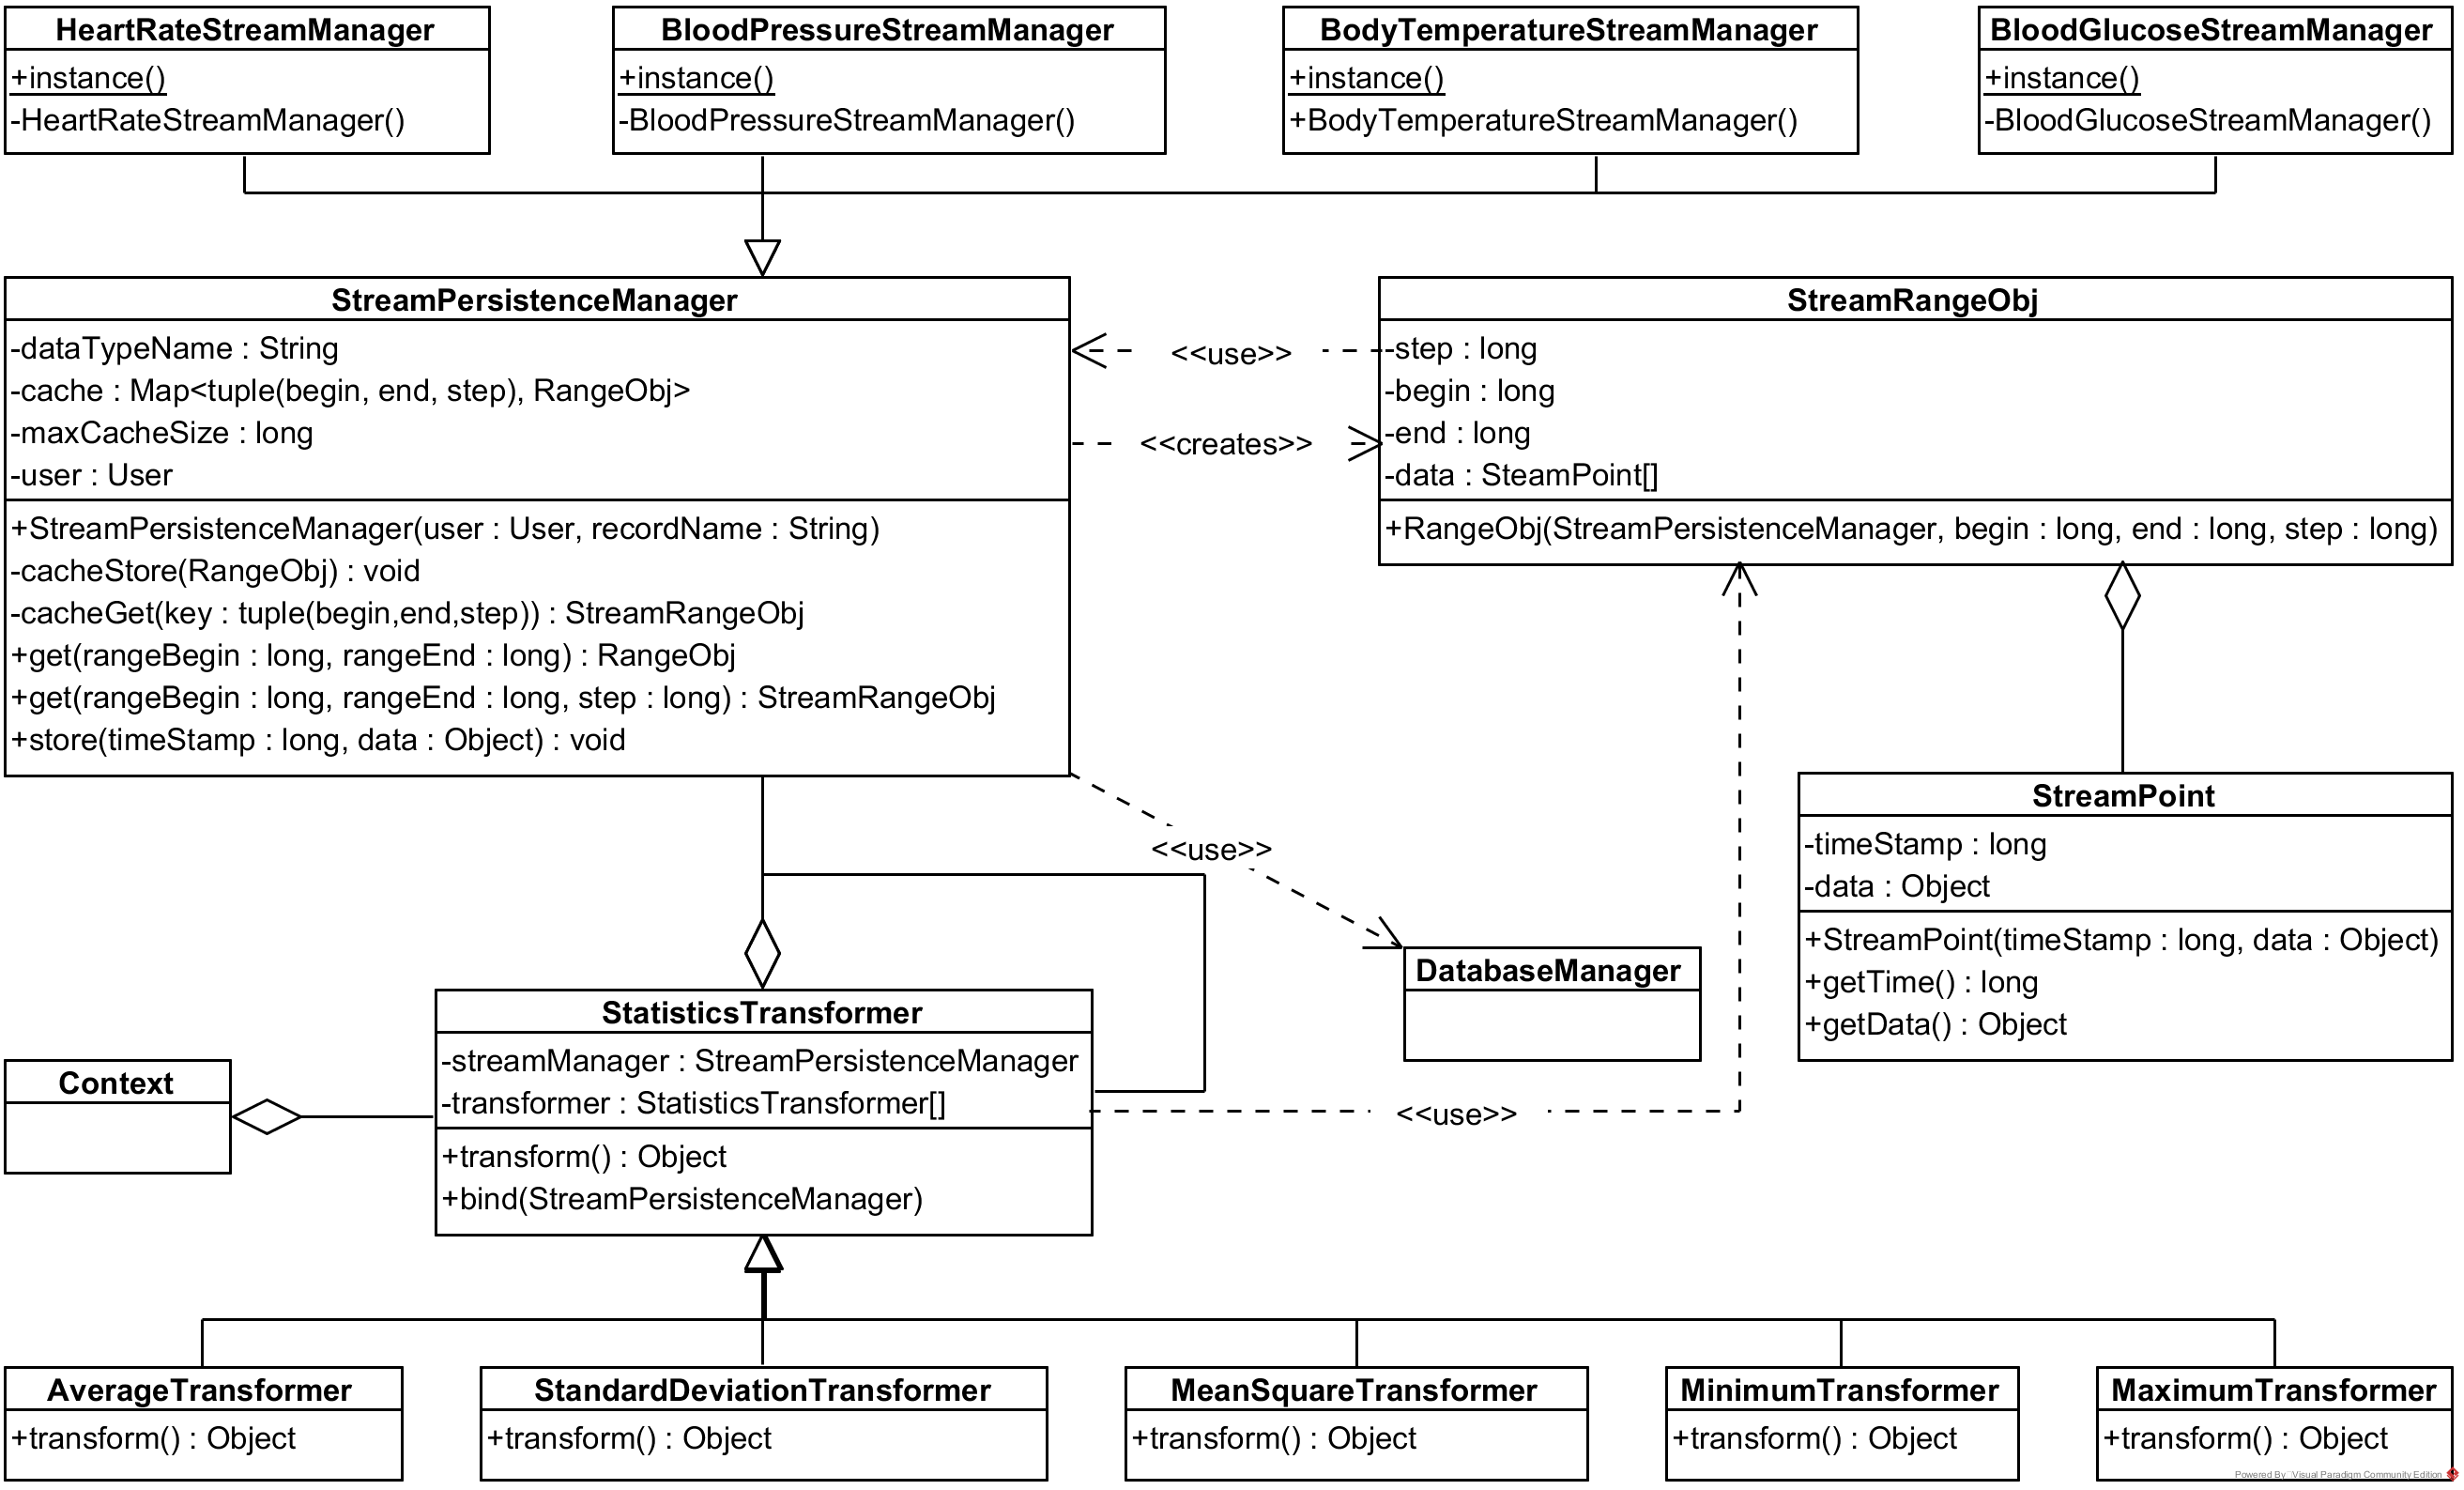
\includegraphics[width=15cm, height=10cm]{StatisticsSubsystem/statisticsClassDiagram.png}
\end{figure}
\end{center}
\subsection*{\textbf{Classes And Design Patterns}}

\subsubsection*{\textbf{StreamPersistenceManager:}}
This class will assume the responsibility of storing collected data streamed from the RaspberryPI. It will also provide a interface to access said data in a robust manner, such that loose coupling can be achieved with regrades to modules that will transform said data into various representations. A range of collected data may for example be sufficiently queried via the interface.

The stored data will be bound to a specific user and time-stamp. These values will act as primary keys. Each instance of this manager will only manage a single user paired with a specific data representation. These representations may include, but is not limited to: heart rate, body temperature, and blood pressure.

To maximize code reuse, each instance will be initialized with a string that defines what the saved data represents. To minimize conflicts such as data races and overlapping writes to the database, only one instance must be instantiated over the entire process.

\textbf{Design Patter:}
To accommodate code reuse, this class will implement a \textit{Collections Singleton} pattern. A mapping will be made between the tuple composed of the user and data represents, and the related singleton instance.

\subsubsection*{\textbf{*StreamManager:}}
These classes that have \textit{StreamManager} appended to their names will inherit from \textit{StreamPersistenceManager}, and handle a specific data represents. This will logically partition the various representations to increase code readability and maintainability.

\textbf{Design Patter:}
The \textit{Singleton} pattern is simply extended from the supper class.


\subsubsection*{\textbf{StreamRangeObj:}}
This class will provide robust means to access various data representations. This class will not physically store the stream data, but act as a cache that contains a range of streamed point values. Queries can be satisfied with this class that might need all the streamed data points over a period of time.

The data may be queried with a specified resolution, e.g. only every second value in the series. This will be determined by the step size.


\subsubsection*{\textbf{StreamPoint:}}
This class will represent each stream data point as a pair, composed of the time-stamp and value.


\subsubsection*{\textbf{StatisticsTransformer:}}
This is an abstract class that provide the interface to transform various stream data into meaningful statistical values. a specific \textit{StreamPersistenceManager} class may be bound at runtime, so that a sigle instance of this class can potentially compute the statistics for a variety of data representations and an array of different users.

\textbf{Design Patter:}
\begin{enumerate}
	\item Strategy: will be used to maximize code reuse
	\item Decorator: will be used to improve modularity and empower the concrete classes to reuse existing \textit{StatisticsTransformer} classes to speed up development.
\end{enumerate}













